% Created 2017-04-14 Fri 16:06
% Intended LaTeX compiler: pdflatex
\documentclass[11pt]{article}
\usepackage[utf8]{inputenc}
\usepackage[T1]{fontenc}
\usepackage{graphicx}
\usepackage{grffile}
\usepackage{longtable}
\usepackage{wrapfig}
\usepackage{rotating}
\usepackage[normalem]{ulem}
\usepackage{amsmath}
\usepackage{textcomp}
\usepackage{amssymb}
\usepackage{capt-of}
\usepackage{hyperref}
\usepackage{indentfirst}
\author{James Nhan, Matt Koenig, Zackery Lovisa, Thien Le}
\date{\textit{<2017-02-24 Fri>}}
\title{Augmented Escape}
\hypersetup{
 pdfauthor={James Nhan, Matt Koenig, Zackery Lovisa, Thien Le},
 pdftitle={Augmented Escape},
 pdfkeywords={},
 pdfsubject={},
 pdfcreator={Emacs 25.1.1 (Org mode 9.0.3)}, 
 pdflang={English}}
\begin{document}

\maketitle
\pagebreak

\section{{\bfseries\sffamily TODO} Story}
\label{sec:org0c412ad}
A mysterious group known only as \emph{The Company} is behind a major conspiracy that will lead to world domination, and you know too much about them. You are being hunted, but death is not your destiny. \emph{The Company} believes anyone can be convinced to join them, and you're no different. They've captured and brough you to a remote location to teach compliance. You will be subjected to various forms of brainwashing and torture techniques. Will you succumb to \emph{The Company}'s will, or will you dash their plans and take them out from inside?

\section{Characters}
\label{sec:org199a281}
\subsubsection{Axshun Jaxxon}
\label{sec:org7d84e9c}

\begin{enumerate}
\item Personality
\label{sec:org7c60101}
Axshun Jaxxon is a rash individual. He is the Leroy Jenkins of Augmented Escape. He uses brute force and brawn over brains. He leaps before he looks. He also loves fried chicken. He may not always get the job done, but at least he's got chicken.

\item Appearance
\label{sec:org54ca9d0}
He has big muscles. He stands 6'6", weighs 280 pounds, is bald, has a goatee, and has one metal pauldron over his right shoulder. The pauldron has a dragon embossment on it. He has tan skin from farming all day. He has no shirt. He has firefighter pants with one leg burnt off at the knee. He wears combat boots.

\item Backstory
\label{sec:orga2a1b95}
He is a firefighter that farms chickens in his free time because he likes chicken. Axshun Jaxxon receives a call from Bearsford, South Dakota dispatch. He is sent on a rescue mission. After rescuing the baby chicks in the farm house, he is alerted to the presence of a child. The child is trapped in the farm house loft. The fire burns so hot and brightly, that his firefighter pants catch flame, resulting in the scorch makes on his left pantleg. A wooden beam from the farm house falls onto his head. He is knocked out cold. Ten days later, he awakes in a sick and twisted game of escaping \emph{The Company}.
\end{enumerate}

\subsubsection{Ben Benson}
\label{sec:org41d29ad}

\begin{enumerate}
\item Personality
\label{sec:org3710707}
Ben Beson is an extremely conservative man born in the secluded areas of Louisiana. He is reserved and quiet. He is cool and calculating. However, when pushed beyond his limits, he is prone to extremely violent outbursts. Whenever possible, Ben Benson will use subterfuge to defeat his enemies. He is the exact opposite of Axshun Jaxxon.

\item Appearance
\label{sec:orgb331019}
He is a mature, white man that wears button up shirts with sweaters. He near sighted and wears glasses. Fluffy brown hair. He is 5'4" and weighs 120 pounds and has no athletic abilities.

\item Backstory
\label{sec:org05e1e5a}
Ben Benson is a Chemistry teacher by trade. In his spare time, he enjoys working at the local car wash. One day, he gets into an argument with his wife, Skylar, over pizza toppings. He gets so angry, he takes their pizza and throws it outside. It lands on their neighbor's house. The next day, a student accidentally mixes the wrong chemicals during the lab and creates mustard gas. This results in an explosion that knocks Ben Benson out. He is taken to the nurse's office. It just so happens that the nurse is an agent of \emph{The Company}. She takes this chance to abduct the genius Chemistry teacher. He wakes up caught in a web of deception and lies. Can he escape the room?
\end{enumerate}

\subsubsection{Yoki Warrior}
\label{sec:org399421c}

\begin{enumerate}
\item Personality
\label{sec:orgfe5d8df}
She is a detective, curious by nature. She is a lone with a serious attitude. She can be insenstive to others' plights. She clean, thorough, detailed oriented, and perfectionist. She has depression because of the extinction of her tribe and the disappearance of her lover. Despite her perfectionst attitude, she despises cyborg technology. She especially hates cyborg technology, as she sees it as an abomination and imperfect.

\item Appearance
\label{sec:orgab7f6a8}
She has light brown skin and long silky hair She wears traditional Native American clothing. Her hair is black and her eyes are also black. As a young woman, she stands 5'3" and weighs 97 pounds. Due to her cyborg reconstruction, her left arm is made of titanium steel alloys. She has an implanted left eye that can perceive ultraviolet and infrared light.

\item Backstory
\label{sec:orgafb0c32}
After single combat with a cyborg bear, she falls unconscious from her grievous wounds. Her noble fighting garnered the attention of the omnipresent \emph{Company}. This prompted them to abduct her into their program. Due to her body being mangled beyond recognition, \emph{The Company} invested \$4 million dollars to rebuild her as cyborg. She is now the thing she hates most: a cyborg.
\end{enumerate}

\subsubsection{The Company}
\label{sec:org8ef1938}

\begin{enumerate}
\item Backstory
\label{sec:org118bb5d}
In 2018, World War III broke out. Nuclear war raged on for 15 years, destroying the vast majority of the planet and decimating the population to the hundreds of thousands. In the aftermath, a reconstructed, cyborg President Nixon gathered the remnants of the Illuminati and the Free Masons. The resulting merger is \emph{The Company}. Biding their time, they gathered influence over the years. Now, in the year 2142, \emph{The Company} has complete anonymous control over the American world government, granting them free reign over North America.

\item Goals
\label{sec:orgee58dfa}
\emph{The Company} currently olds captive the continent of North America. Their ultimate goal is to overthrow the other two remaining world governments: China, and the Afindican Warlords as well as the rogue rebels in Antarctica: The Nomads.

\item Influence and Power
\label{sec:org50465f0}
Having complete anonymous control over North America gives them access to unlimited natural resources. Using their cyborg technology, they have implanted control chips into the newest generation, giving them access to the largest standing army still in existence today. They utilize \emph{The Program} to recruite the best of the best of the previous generation, such as Axshun Jaxxon, Ben Benson, and Yoki Warrior.
\end{enumerate}

\subsubsection{{\bfseries\sffamily TODO} Afindican Warlords}
\label{sec:org8ccb676}

\begin{enumerate}
\item Backstory
\label{sec:org31a25bb}

\item Goals
\label{sec:org14fe4b2}

\item Influence and Power
\label{sec:org6e51afb}
\end{enumerate}

\subsubsection{{\bfseries\sffamily TODO} The Chinese Conglomerate}
\label{sec:org986e795}

\begin{enumerate}
\item Backstory
\label{sec:org41e2597}

\item Goals
\label{sec:org306e92b}

\item Influence and Power
\label{sec:orga63481c}
\end{enumerate}

\subsubsection{{\bfseries\sffamily TODO} The Nomads}
\label{sec:orgbab6b18}

\begin{enumerate}
\item Backstory
\label{sec:org0ee2b0d}

\item Goals
\label{sec:org5eb7ed1}

\item Influence and Power
\label{sec:org0295410}
\end{enumerate}

\subsubsection{{\bfseries\sffamily TODO} Mittens}
\label{sec:orgf3a51a5}
\begin{itemize}
\item Mystical cat.
\item Appears in dire situations to provide help.
\item Requires the player to answer a simple riddle before willing to provide a hint.
\item Has a very playful attitude, making light of the player's current situation
\end{itemize}

\section{Core Gameplay}
\label{sec:orge5f5163}
\subsection{{\bfseries\sffamily TODO} Mechanics}
\label{sec:orgeff7d06}
\begin{itemize}
\item Single player.
\item Puzzle solving.
\item Room is mapped by the HoloLens and augmented to match a scenario.
\item 3-4 puzzles placed around the room randomly.
\item Each puzzle gives a piece of the answer to escaping the current room.
\item Puzzles will be interactable 3D objects in augmented reality.
\item Once all puzzles of a room are solved, their answers can be entered into the door (keys, lock code).
\item Some puzzles and rooms will have random components in order to prevent "trial and error" attempts through the game.
\item Entering a wrong room answer will result in a \textbf{1 minute penalty}.
\item Players will have \textbf{1 hour} to solve all puzzles in all rooms.
\item Scenarios will contain \textbf{3 rooms} each.
\item All rooms must be completed within the time limit to complete the scenario.
\item Upon advancing to a new room in the game, the HoloLens will remap the current room the player is in.
\begin{itemize}
\item The player does not have to change rooms themselves.
\end{itemize}
\item Upon successful completion of the scenario, a story prompt will be shown to the player describing the events that follow the escape.
\item At \textbf{50 minutes} remaining, Mittens will appear to give the players a hint in case they're stuck.
\begin{itemize}
\item If a hint is given, Mittens will disappear and reappear at \textbf{40}, \textbf{30}, \textbf{25}, \textbf{15}, and \textbf{10} minutes remaining.
\item Hints will be consistent for each playthrough of the same scenario.
\end{itemize}
\end{itemize}

\subsection{{\bfseries\sffamily TODO} Goals}
\label{sec:org2d08b10}
\begin{itemize}
\item Players win the game if they manage to escape the scenario within an hour.
\item After winning, an expository paragraph will be shown to the player to describe what happens following the escape.
\item Players lose if time expires.
\item After losing, an expository paragraph will be shown to the player to describe what happens to them after their escape fails.
\end{itemize}

\subsection{{\bfseries\sffamily TODO} Hints}
\label{sec:org99b8d17}
\begin{itemize}
\item Mittens can give the player several types of hints after the player answers a riddle.
\begin{itemize}
\item \textbf{Remove Decoys}: Remove all or some of the decoys in the room.
\item \textbf{Puzzle Explanation}: Explain part of a puzzle to make it easier for the player to solve.
\item \textbf{Answer Location}: Place a glow on an object required for a puzzle.
\end{itemize}
\end{itemize}

\section{Puzzle Types}
\label{sec:orge7e6ee3}
\subsection{{\bfseries\sffamily TODO} Acrostic}
\label{sec:org7482032}
Hint words with numbers under each letter that map to a phrase.

\subsection{{\bfseries\sffamily TODO} Rope Chain}
\label{sec:org4c9f4f1}
There will be four \textbf{20 foot} ropes each with four pegs spaced at different distances apart attached along the rope. Only one rope will have the exact peg separation required to insert each peg into four anchored podiums across the room.

\begin{center}
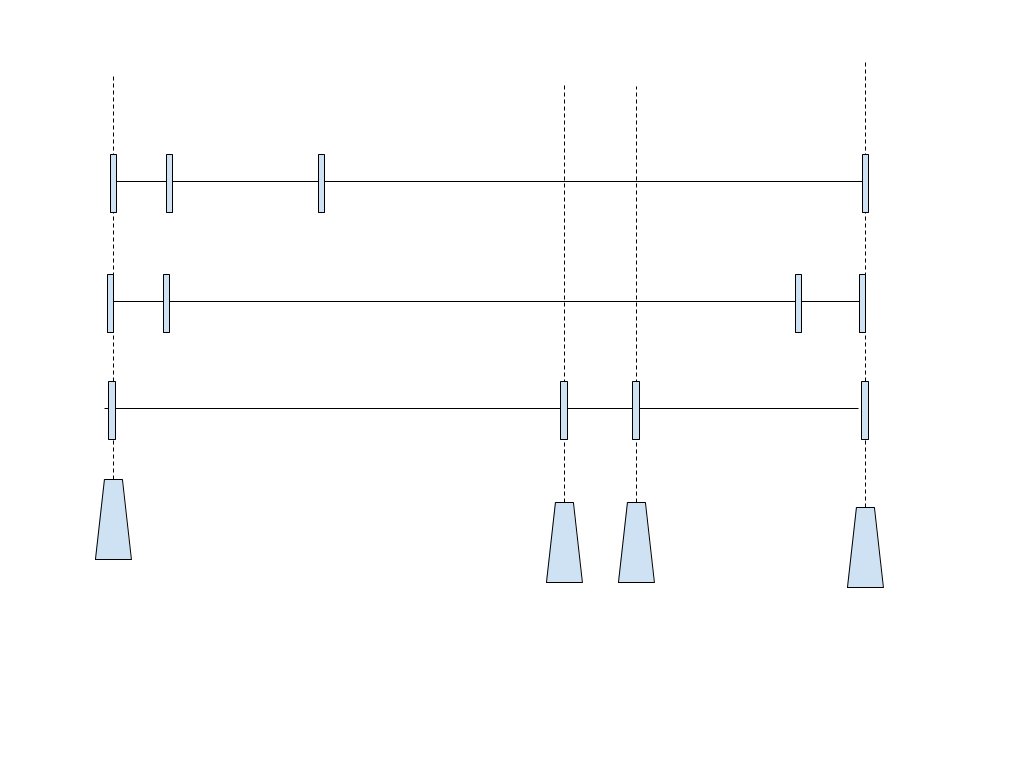
\includegraphics[width=.9\linewidth]{./img/pt-rc-001.png}
\captionof{figure}{\label{fig:org26a0969}
An example of the ropes, pegs, and podiums.}
\end{center}

\subsection{{\bfseries\sffamily TODO} Block and Key}
\label{sec:org6ee593a}
There will be six \textbf{1 foot} cubes spread across the room. The player will need to place and orient these blocks on a pedestal to create an image by aligning the engravings on each cube. The opposite side of the cube array will then reveal an answer required to escape the room.

\subsection{{\bfseries\sffamily TODO} Cryptogram}
\label{sec:orgd5eec0e}
Encrypted messages that need to be put through a cipher in order to be easily read.

\subsection{{\bfseries\sffamily TODO} Connect the Dots}
\label{sec:org9ad1b01}
Images drawn may be of other objects in the room. Different shaped dots (e.g. square vs. circle) will connect to make different images. A key will be placed in the room to indicate which dots make the correct image.

\subsection{{\bfseries\sffamily TODO} Statues/Totems}
\label{sec:org02e0e7b}
\textbf{3-4} statues or obelisks with images need to be positioned in a particular way to unlock an answer. There will be an image depicting how to orient the statues around the room.

\section{References}
\label{sec:orgb5f43e7}
\begin{itemize}
\item \href{https://en.wikipedia.org/wiki/Acrostic\_(puzzle)}{Acrostic} - Wikipedia entry.
\item \href{https://en.wikipedia.org/wiki/Cryptogram}{Cryptogram} - Wikipedia entry.
\item \href{http://www.bloodandbones.com/ph12sim/types.htm}{Puzzle Idea List} - A list of puzzle ideas.
\item \href{http://www.accelerated-ideas.com/news/uncharted-4-chapter-1-2-puzzle-solution-rotating-balls.aspx}{Rotating balls and Symbols} - A description of the rotating balls and symbols puzzle from Uncharted 4.
\item \href{http://www.gameshampoo.com/magazine/articles/24/uncharted-3-all-puzzle-solutions.html}{Uncharted 3 All Puzzles} - All of the puzzles in Uncharted 3.
\end{itemize}
\end{document}
